\documentclass[
	% -- opções da classe memoir --
	11pt,				% tamanho da fonte
	oneside,			% impressão só-frente
	a4paper,			% tamanho do papel
	% -- opções da classe abntex2 --
	chapter=TITLE,		% títulos de capítulos em maiúsculas
	% -- opções do pacote babel --
	english,			% idioma adicional para hifenização
	brazil,				% o último idioma é o principal
	]{abntex2}

% ------------------------------------
% PACOTES
% ------------------------------------

% Pacotes fundamentais
\usepackage{times}			% Times New Roman
\usepackage[T1]{fontenc}		% Seleção de códigos de fonte
\usepackage[utf8]{inputenc}		% Codificação do documento
\usepackage{indentfirst}		% Indenta o primeiro parágrafo de cada seção
\usepackage{xcolor}				% Controle de cores
\usepackage{graphicx}			% Inclusão de gráficos
\usepackage{microtype} 			% Melhorias de justificação
\usepackage{booktabs}			% \toprule, \midrule, \bottomrule
\usepackage{adjustbox}			% Ajuste de tabelas largas
\usepackage{array}				% Colunas formatadas (>{\ttfamily}, etc.)
\usepackage{tabularx}			% Colunas X
\usepackage{enumitem}			% Controle de listas

% Formato específico IFSULDEMINAS.
% ATENÇÃO: se você NÃO tem o arquivo IFSULDEMINAS.sty no projeto,
% comente a linha abaixo; caso contrário, a compilação falhará.
\usepackage{IFSULDEMINAS}

% Pacotes adicionais (anexo do modelo de folha de identificação)
\usepackage{multicol}
\usepackage{multirow}

% Pacotes adicionais do Modelo Canônico do abnTeX2
\usepackage{lipsum}

% Pacotes de citações
\usepackage[brazilian,hyperpageref]{backref}
\usepackage[alf]{abntex2cite}

% Configuração de listas
\setlist{itemsep=2pt}

% ------------------------------------
% CONFIGURAÇÕES DE PACOTES
% ------------------------------------

% --- backref ---
\renewcommand{\backrefpagesname}{Citado na(s) página(s):~}
\renewcommand{\backref}{}
\renewcommand*{\backrefalt}[4]{%
	\ifcase #1 %
		Nenhuma citação no texto.%
	\or
		Citado na página #2.%
	\else
		Citado #1 vezes nas páginas #2.%
	\fi}%

% --- Comando \todo ---
\newcommand{\todo}[1]{\textcolor{red}{[\textbf{A FAZER:} #1]}}

% --- Comando \ficha ---
\newcommand{\ficha}[4]{%
\begin{center}\small
\begin{tabularx}{\textwidth}{>{\bfseries}p{3.2cm}X}
\toprule
Tabela & #1 \\
Cada linha é & #2 \\
Quantas linhas & #3 \\
De onde vem & #4 \\
\bottomrule
\end{tabularx}
\end{center}}

% ------------------------------------
% DADOS DO DOCUMENTO
% ------------------------------------

\titulo{Tema do artigo\\}
\autor{Eric Rodrigues das Chagas - 12623971\\ Danillo Mendes Santiago - 10414592}
\local{São Carlos}
\data{2026}

% ------------------------------------
% APARÊNCIA DO PDF
% ------------------------------------

\definecolor{blue}{RGB}{41,5,195}

\makeatletter
\hypersetup{
		pdftitle={\@title},
		pdfauthor={\@author},
		pdfsubject={},
		pdfcreator={LaTeX with abnTeX2},
		pdfkeywords={abnt}{latex}{abntex}{abntex2}{relatório técnico},
		colorlinks=true,
		linkcolor=black,
		citecolor=blue,
		filecolor=magenta,
		urlcolor=blue,
		bookmarksdepth=4
}
\makeatother

% ------------------------------------
% ESPAÇAMENTOS
% ------------------------------------

\setlength{\parindent}{1.4cm}
\setlength{\parskip}{0.3cm}

\makeindex

% ====================================
% INÍCIO DO DOCUMENTO
% ====================================
\begin{document}

\selectlanguage{brazil}
\frenchspacing

% ------------------------------------
% ELEMENTOS PRÉ-TEXTUAIS
% ------------------------------------
\imprimircapa

\pdfbookmark[0]{\contentsname}{toc}
\tableofcontents*
\cleardoublepage

% ------------------------------------
% ELEMENTOS TEXTUAIS
% ------------------------------------
\textual

\chapter{Capítulo 01}
\label{cap:cap01}

%----------------------------------------------------------------------
\section{[Tema]}
\label{sec:tema}

\subsection{[Subtema]}
\label{subsec:subtema1}

Lorem ipsum dolor sit amet, consectetur adipiscing elit, sed do eiusmod tempor incididunt ut
labore et dolore magna aliqua. Ut enim ad minim veniam, quis nostrud exercitation ullamco laboris
nisi ut aliquip ex ea commodo consequat. Duis aute irure dolor in reprehenderit in voluptate velit
esse cillum dolore eu fugiat nulla pariatur. Excepteur sint occaecat cupidatat non proident, sunt
in culpa qui officia deserunt mollit anim id est laborum.

%----------------------------------------------------------------------
\subsection{[Subtema]}
\label{subsec:subtema2}

Lorem ipsum dolor sit amet, consectetur adipiscing elit, sed do eiusmod tempor incididunt ut
labore et dolore magna aliqua. Ut enim ad minim veniam, quis nostrud exercitation ullamco laboris
nisi ut aliquip ex ea commodo consequat. Duis aute irure dolor in reprehenderit in voluptate velit
esse cillum dolore eu fugiat nulla pariatur. Excepteur sint occaecat cupidatat non proident, sunt
in culpa qui officia deserunt mollit anim id est laborum.
\chapter{Experimento prático para classificação de resultado de processos civis no recorte da Lei [...]}
\label{cap:conc}

% =====================================================================
\section{Metodologia}
% =====================================================================

\subsection*{A pergunta}

Se escrevermos a lei como um programa de computador (um ``juiz virtual'' que só segue
regras), as decisões ficam livres de viés? A hipótese do trabalho é que não: para
transformar a lei em regras, alguém precisa preencher o que a lei deixa em aberto, e
essas escolhas mudam o resultado.

\subsection*{O caso estudado: o tráfico privilegiado}

O crime de tráfico (art.~33 da Lei de Drogas, Lei 11.343/2006) tem pena de 5 a 15 anos.
O parágrafo 4º desse artigo permite \textbf{reduzir a pena de 1/6 a 2/3} quando o réu
cumpre quatro condições ao mesmo tempo:
\begin{enumerate}
  \item é \textbf{primário} (não é reincidente);
  \item tem \textbf{bons antecedentes};
  \item \textbf{não se dedica a atividades criminosas};
  \item \textbf{não faz parte de organização criminosa}.
\end{enumerate}
Com a redução máxima, uma pena de 5 anos cai para 1 ano e 8 meses, em regime aberto.
Sem a redução, fica em 5 anos ou mais, em regime semiaberto ou fechado.
Escolhemos esse ponto porque é o pedido mais comum nos recursos e porque a lei
\textbf{não diz} duas coisas: o que significa ``dedicar-se a atividades criminosas'' e
como escolher a fração entre 1/6 e 2/3 (manda só ``considerar a natureza e a quantidade
da droga'').

\subsection*{De onde vieram os dados}

\begin{itemize}
  \item \textbf{Decisões do Superior Tribunal de Justiça (STJ)}, publicadas pelo próprio
        tribunal em arquivos abertos, um por mês. Usamos as duas turmas que julgam
        crimes (5ª e 6ª Turma), publicadas de janeiro a outubro de 2025 e de junho a
        agosto de 2026 (13 meses; os meses intermediários foram descartados, como explica a
        seção~\ref{sec:dados}).
  \item \textbf{A ficha de cada processo} no site do STJ: quem são as partes, os recursos
        apresentados e o texto completo das decisões (em PDF).
  \item \textbf{O texto da lei} em vigor (Lei de Drogas e Código Penal).
\end{itemize}

Ficaram de fora os casos que não tratam de uma condenação por tráfico: prisões antes da
sentença, execução da pena, atos de adolescentes e o crime de associação sem tráfico.

\subsection*{As tabelas de dados}

O trabalho usa quatro tabelas. Para cada uma, dizemos o que é uma linha, quantas
linhas há e quais colunas (variáveis) ela tem.

\paragraph*{Tabela 1 -- Decisões do STJ (base grande).}
\ficha{\texttt{dados/ementas\_t5.csv} e \texttt{dados/ementas\_t6.csv}}
      {um processo de tráfico, na decisão mais recente do período}
      {5.778 processos (3.396 da 5ª Turma e 2.382 da 6ª). Em 5.323 deles, quem recorreu foi a defesa.}
      {lida por um programa a partir do resumo oficial da decisão (a ``ementa''), sem leitura humana}

\begin{center}\small
\begin{tabular}{>{\ttfamily}l p{6.6cm} p{5cm}}
\toprule
\normalfont\bfseries Coluna & \bfseries O que diz & \bfseries Valores possíveis \\
\midrule
turma & qual turma julgou & 5ª ou 6ª \\
relator & o ministro responsável pelo processo & 15 nomes \\
mes\_publicacao & o mês do arquivo em que a decisão saiu & 2025-01 a 2026-08 \\
classe & o tipo de recurso & HC, RHC, AREsp, REsp \\
objeto & o assunto principal do pedido & § 4º, busca ilegal, pena, \ldots \\
recorrente & quem recorreu & defesa ou Ministério Público \\
dispositivo & o que o tribunal decidiu & deu, negou, não conheceu, \ldots \\
resultado\_reu & o resultado \emph{para o réu} & favorável, parcial, desfavorável \\
barreiras & regras processuais usadas para não analisar o pedido & Súmula 7, Súmula 182, \ldots \\
marcadores & expressões sobre a pessoa ou o lugar & ``vulgo'', facção, ``local conhecido'', \ldots \\
votacao & se a decisão foi unânime & unânime ou por maioria \\
relator\_vencido & se o relator perdeu a votação & sim ou não \\
\bottomrule
\end{tabular}
\end{center}

O programa que lê as ementas foi conferido contra os processos lidos por inteiro: acertou
o resultado para o réu em 32 de 33 processos da amostra da 5ª Turma, 29 de 30 da 6ª e 23 de
27 da base do §~4º. Os erros são quase sempre vitórias parciais obtidas antes, na decisão
individual do relator, que a ementa do julgamento final não menciona.

\paragraph*{Tabela 2 -- Amostras lidas por inteiro.}
\ficha{\texttt{dados/amostra\_casos.csv} (5ª Turma) e \texttt{dados/amostra\_t6\_casos.csv} (6ª Turma)}
      {um réu}
      {5ª Turma: 42 réus (34 dentro do recorte). 6ª Turma: 43 réus (31 dentro do recorte). Mais 14 casos escolhidos à mão para contraste.}
      {40 processos sorteados por turma, com o mesmo número por relator; o texto completo foi lido com apoio de um programa de IA, seguindo um roteiro escrito, e parte foi conferida à mão}

As colunas descrevem os \textbf{fatos} (droga, quantidade, como foi a abordagem policial,
antecedentes) e \textbf{o que cada instância decidiu} (juiz, Tribunal de Justiça e STJ).

\paragraph*{Tabela 3 -- Base do § 4º.}
\ficha{\texttt{dados/amostra\_p4\_casos.csv}}
      {um réu que pediu a redução do § 4º}
      {30 réus (27 processos) até agora, de 4 relatores: Sebastião Reis (22 réus), Maria Marluce (3), Ribeiro Dantas (3) e Rogerio Schietti (2). O plano prevê 99 processos de 10 relatores.}
      {todas as vitórias da defesa e 8 derrotas sorteadas por relator; texto completo lido com o mesmo roteiro}

Esta tabela foi feita para ter os fatos que a lei exige. Principais colunas:
droga, quantidade em gramas, primário, reincidente, maus antecedentes, atos infracionais
(quando adolescente), processos em andamento, condenação por associação, indícios de
dedicação (balança, celular, investigação prévia\ldots), o que o juiz, o TJ e o STJ decidiram
sobre a redução e por quê.

\paragraph*{Tabela 4 -- Entrada do juiz virtual.}
\ficha{\texttt{prolog/fatos\_casos.pl} (gerada pelo programa \texttt{scripts/gerar\_fatos.py})}
      {um réu em que a redução do § 4º foi discutida}
      {71 réus: 30 da base do § 4º, 17 da amostra da 5ª Turma, 13 da 6ª e 11 dos casos de contraste}
      {as Tabelas 2 e 3, convertidas para o formato que o juiz virtual lê}

A Tabela~\ref{tab:cobertura} mostra um ponto importante: \textbf{muitos dos fatos que a lei
exige não aparecem nas decisões}. A primariedade, por exemplo, só é informada em 33 dos 71
réus.

\begin{table}[h]
\centering\small
\caption{Em quantos dos 71 réus cada fato aparece no texto das decisões.}
\label{tab:cobertura}
\begin{tabular}{lr}
\toprule
Fato & Réus em que aparece \\
\midrule
Tipo de droga & 58 \\
Algum indício de dedicação (balança, celular, arma\ldots) & 55 \\
Quantidade em gramas & 47 \\
Se é primário & 33 \\
Antecedentes & 23 \\
Se é reincidente & 16 \\
Data do fato (completa) & 14 \\
Atos infracionais & 8 \\
Processos em andamento & 4 \\
\bottomrule
\end{tabular}
\end{table}

\subsection*{O juiz virtual (árvore A)}

O juiz virtual é um programa em Prolog (\texttt{prolog/arvore\_a.pl}), uma linguagem em que se
escrevem regras do tipo ``se \ldots\ então \ldots''. Para cada réu, ele faz estas perguntas:
\begin{enumerate}
  \item O fato aconteceu depois da Lei de Drogas de 2006? Se não, a redução não existe.
  \item O réu é primário?
  \item Tem bons antecedentes?
  \item Dedica-se a atividades criminosas?
  \item Faz parte de organização criminosa?
  \item Se passou em todas: qual fração aplicar (de 1/6 a 2/3)?
  \item Qual é a pena final, o regime e se dá para trocar a prisão por pena alternativa?
\end{enumerate}
As perguntas 2, 3 e 5 dependem só dos fatos. As perguntas 4 e 6 dependem de
\textbf{escolhas}, porque a lei não diz como respondê-las. No programa, cada escolha virou
um ajuste explícito, e um conjunto de ajustes forma uma \textbf{leitura} da lei.
Criamos três leituras (Tabela~\ref{tab:perfis}). Elas foram inspiradas em decisões reais
que estudamos, mas não pretendem representar nenhum ministro.

\begin{table}[h]
\centering\small
\caption{As escolhas que a lei não faz, e as três leituras usadas.}
\label{tab:perfis}
\begin{adjustbox}{max width=\textwidth}
\begin{tabular}{lccc}
\toprule
Escolha & Garantista & Intermediária & Restritiva \\
\midrule
Muita droga indica dedicação ao crime? & não & sim & sim \\
Muita droga, sozinha, basta para negar? & não & não & sim \\
O que é ``muita'' maconha / cocaína & --- & 10 kg / 1 kg & 1 kg / 100 g \\
Atos infracionais de quando era adolescente contam? & não & até 3 anos antes & até 5 anos antes \\
Processos ainda em andamento contam? & não & não & sim \\
Condenação antiga (mais de 5 anos) é esquecida? & sim & não & não \\
Quais indícios de dedicação contam & arma, facção & + balança, celular, & + denúncias, ``local \\
 & & investigação, transporte & conhecido'', dinheiro \\
Quantos indícios bastam & 2 & 2 & 1 \\
\bottomrule
\end{tabular}
\end{adjustbox}
\end{table}

Há ainda uma escolha que vale para todas as leituras: \textbf{o que fazer quando um fato não
aparece no processo}. Pode-se decidir a favor do réu (``na dúvida, a favor do réu'') ou
contra ele (``cabe à defesa provar''). Testamos as duas opções.

Para isolar o efeito da redução, o juiz virtual parte sempre da pena mínima de 5 anos e só
aplica a redução e o aumento por circunstâncias especiais (como tráfico perto de escola).
Ele também explica cada decisão: quais condições falharam e quais indícios foram usados.

\subsection*{A árvore aprendida (árvore B)}

A árvore B não foi escrita por nós: um programa (\texttt{scikit-learn}) a \textbf{aprendeu}
olhando as decisões reais. Ela aprende uma sequência de perguntas de sim ou não que melhor
separa os casos em que a defesa ganhou dos casos em que perdeu. Depois, a árvore é
convertida em regras Prolog (\texttt{prolog/arvore\_b.pl}).
\begin{itemize}
  \item \textbf{Linhas usadas:} os 5.323 processos da Tabela 1 em que a defesa recorreu.
        Desses, 308 foram vitórias da defesa.
  \item \textbf{O que ela tenta adivinhar (coluna-alvo):} se a defesa venceu ou perdeu.
  \item \textbf{O que ela pode olhar (colunas de entrada):} turma, relator, tipo de recurso,
        assunto e os marcadores da ementa. Ou seja, só o que se sabia antes do julgamento.
  \item \textbf{O que ela não pode olhar:} as barreiras processuais, a votação e se o relator
        perdeu, porque essas informações já fazem parte da decisão. Usá-las seria ``colar''
        a resposta.
  \item \textbf{Tamanho:} no máximo 4 perguntas seguidas, e cada resposta final precisa valer
        para pelo menos 10 processos.
  \item \textbf{Duas versões:} uma pode usar o relator e a turma; a outra não.
\end{itemize}
O objetivo não é acertar muito. Como a defesa perde em 94\% dos casos, um programa que
sempre diz ``perde'' acerta 94\% sem aprender nada. O que interessa é \textbf{quais
perguntas} ela aprende a fazer.

\subsection*{Como verificamos os programas}

O juiz virtual passou por 26 testes com réus inventados, um para cada regra (por exemplo:
``réu reincidente nunca recebe a redução'' e ``um fato de 2005 não tem redução''). A árvore B
foi testada para garantir que as regras em Prolog decidem exatamente como o modelo
aprendido, nos 5.323 processos.

% =====================================================================
\section{Os dados em números}
\label{sec:dados}
% =====================================================================
% Números gerados por scripts/contagens.py (na raiz do projeto), a partir de
% dados/ementas_t5.csv, dados/ementas_t6.csv, dados/meses.csv e das amostras lidas por inteiro.

Antes dos experimentos, vale olhar os dados com contagens simples. Salvo indicação
contrária, os números são da Tabela 1 (decisões do STJ): 5.778 processos de tráfico
julgados pela 5ª e pela 6ª Turma e publicados em 13 meses (janeiro a outubro de 2025 e junho
a agosto de 2026).

\subsection*{Quantos processos e de que tipo}

A 5ª Turma julgou 3.396 processos e a 6ª, 2.382. O tipo de recurso mais comum é o
\emph{habeas corpus} (HC), seguido do agravo em recurso especial (AREsp), que é o recurso
usado quando o tribunal estadual nega a subida do recurso especial.

\begin{table}[h]
\centering\small
\caption{Processos por turma e tipo de recurso.}
\label{tab:dados-classe}
\begin{tabular}{lrrr}
\toprule
Tipo de recurso & 5ª Turma & 6ª Turma & Total \\
\midrule
\emph{Habeas corpus} (HC) & 1.679 & 1.350 & 3.029 (52\%) \\
Agravo em recurso especial (AREsp) & 1.168 & 674 & 1.842 (32\%) \\
Recurso especial (REsp) & 474 & 293 & 767 (13\%) \\
Outros (RHC, RMS e outros) & 75 & 65 & 140 (2\%) \\
\midrule
Total & 3.396 & 2.382 & 5.778 \\
\bottomrule
\end{tabular}
\end{table}

O assunto mais frequente é justamente a redução do § 4º, presente em um terço dos
processos (Tabela~\ref{tab:dados-assunto}).

\begin{table}[h]
\centering\small
\caption{Assunto principal do pedido.}
\label{tab:dados-assunto}
\begin{tabular}{lrrr}
\toprule
Assunto & 5ª Turma & 6ª Turma & Total \\
\midrule
Redução do § 4º (tráfico privilegiado) & 1.192 & 739 & 1.931 (33\%) \\
Busca policial ilegal (pessoal ou na casa) & 893 & 637 & 1.530 (26\%) \\
Cálculo da pena & 470 & 278 & 748 (13\%) \\
Ser tratado como usuário, e não traficante & 282 & 170 & 452 (8\%) \\
Não ter sido o autor & 169 & 114 & 283 (5\%) \\
Outros & 390 & 444 & 834 (14\%) \\
\bottomrule
\end{tabular}
\end{table}

\subsection*{Quais meses entraram}

O STJ publica um arquivo por mês. Baixamos de janeiro de 2025 a agosto de 2026, mas sete
meses (novembro de 2025 a maio de 2026) ficaram de fora: nesses arquivos há só 8\% a 30\% do
volume habitual de decisões, e a defesa vence em 12\% a 75\% dos recursos, mais do que em
qualquer mês completo (0\% a 22\%). Isso indica que esses arquivos trazem uma seleção de
decisões, e não todas.
A contagem mês a mês está em \texttt{dados/meses.csv}.

A Figura~\ref{fig:taxa-mensal} mostra a taxa de vitória da defesa em cada mês completo. A 5ª
Turma começa 2025 bem acima da 6ª (até 21\% em fevereiro) e, a partir de março, fica quase
sempre abaixo dela. A 6ª Turma oscila em torno de 5\% o tempo todo. A virada da 5ª Turma
coincide com a saída de Daniela Teixeira da relatoria: ela relatou 268 dos 343 recursos da
defesa julgados pela 5ª Turma em janeiro de 2025 e 284 dos 461 em fevereiro, mas só 103 em
março e quase nenhum de abril em diante. A seção seguinte trata dos relatores.

\begin{figure}[h]
\centering
\caption{Recursos da defesa em que ela vence, por mês e turma (só meses completos).}
\label{fig:taxa-mensal}
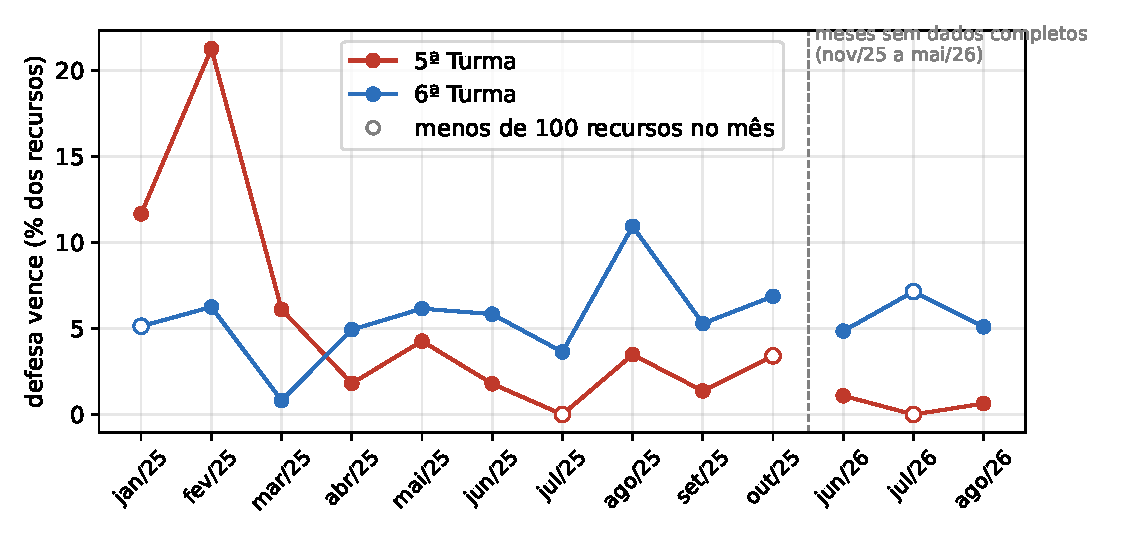
\includegraphics[width=\textwidth]{Imagens/taxa_mensal.pdf}
\legend{Fonte: elaborado pelo autor a partir dos espelhos de acórdãos do STJ. Pontos vazios:
meses com menos de 100 recursos da defesa, em que a taxa varia muito por acaso.}
\end{figure}

\subsection*{Quem recorre e quem ganha}

Em 5.323 processos (92\%) quem recorreu foi a defesa. Para o réu, o resultado foi
desfavorável em 5.066 processos (88\%), favorável em 575 e parcialmente favorável em 137.
Nos recursos da defesa, ela vence em 308 de 5.323 (5,8\%).

A Tabela~\ref{tab:dados-turma} separa as turmas e os anos. Ela mostra algo importante:
\textbf{a diferença entre as turmas não é fixa}. Em 2025, a 5ª Turma dava mais vitórias que
a 6ª; em 2026, passou a dar quase nenhuma. A 6ª Turma ficou estável. O que mudou na 5ª Turma
foi a sua composição, como mostra a próxima seção.

\begin{table}[h]
\centering\small
\caption{Recursos da defesa e vitórias, por turma e ano.}
\label{tab:dados-turma}
\begin{tabular}{llrrr}
\toprule
Turma & Ano & Recursos da defesa & Vitórias & Defesa vence \\
\midrule
5ª Turma & 2025 & 2.247 & 184 & 8,2\% \\
5ª Turma & 2026 & 836 & 7 & 0,8\% \\
6ª Turma & 2025 & 1.582 & 84 & 5,3\% \\
6ª Turma & 2026 & 658 & 33 & 5,0\% \\
\bottomrule
\end{tabular}
\end{table}

\subsection*{Os relatores}

A Tabela~\ref{tab:dados-relator} mostra a taxa de vitória da defesa com cada relator. A
diferença é grande dentro das duas turmas; a chance de ela ser acaso é praticamente nula
(teste qui-quadrado).

A última coluna é a \textbf{margem de erro}: o intervalo em que a taxa ``verdadeira'' do
relator deve estar, com 95\% de confiança (intervalo de Wilson). Ela é larga quando há poucos
processos. Mesmo assim, a faixa de Daniela Teixeira (19\% a 25\%) não chega nem perto da de
nenhum colega da 5ª Turma (todas abaixo de 7\%), e a de Sebastião Reis (6\% a 11\%) fica acima
das de Carlos Pires e Nilsoni de Freitas (até 3\%). Já entre relatores como Reynaldo Soares,
Ribeiro Dantas e Maria Marluce as faixas se sobrepõem: com estes dados, não dá para dizer que
eles decidem de forma diferente.

\begin{table}[h]
\centering\small
\caption{Recursos da defesa e vitórias, por relator (2025 e 2026 somados), com a margem de erro de 95\%.}
\label{tab:dados-relator}
\begin{adjustbox}{max width=\textwidth}
\begin{tabular}{llrrrr}
\toprule
Turma & Relator & Recursos da defesa & Vitórias & Defesa vence & Margem (95\%) \\
\midrule
5ª & Daniela Teixeira (só 2025) & 681 & 150 & 22,0\% & 19,1 a 25,3 \\
5ª & Reynaldo Soares da Fonseca & 547 & 12 & 2,2\% & 1,3 a 3,8 \\
5ª & Ribeiro Dantas & 427 & 10 & 2,3\% & 1,3 a 4,3 \\
5ª & Carlos Cini (convocado, só 2025) & 203 & 7 & 3,4\% & 1,7 a 6,9 \\
5ª & Maria Marluce Caldas (quase só 2026) & 193 & 4 & 2,1\% & 0,8 a 5,2 \\
5ª & Messod Azulay Neto & 557 & 4 & 0,7\% & 0,3 a 1,8 \\
5ª & Joel Ilan Paciornik & 475 & 4 & 0,8\% & 0,3 a 2,1 \\
\midrule
6ª & Sebastião Reis Júnior & 624 & 52 & 8,3\% & 6,4 a 10,8 \\
6ª & Otávio de Almeida Toledo (convocado, só 2025) & 308 & 24 & 7,8\% & 5,3 a 11,3 \\
6ª & Rogerio Schietti Cruz & 299 & 13 & 4,3\% & 2,6 a 7,3 \\
6ª & Og Fernandes & 327 & 14 & 4,3\% & 2,6 a 7,1 \\
6ª & Antonio Saldanha Palheiro & 399 & 14 & 3,5\% & 2,1 a 5,8 \\
6ª & Carlos Pires Brandão (quase só 2026) & 149 & 0 & 0,0\% & 0,0 a 2,5 \\
6ª & Nilsoni de Freitas (convocada, só 2026) & 134 & 0 & 0,0\% & 0,0 a 2,8 \\
\bottomrule
\end{tabular}
\end{adjustbox}
\end{table}

\paragraph*{O caso da 5ª Turma.} Em 2025, a ministra Daniela Teixeira foi relatora de 681
recursos da defesa e deu alguma vitória em 150 (22\%). Os demais relatores da mesma turma, no
mesmo período, deram em 34 de 1.566 (2,2\%). Em 2026 ela não aparece mais como relatora na
5ª Turma, e a taxa da turma caiu de 8,2\% para 0,8\%. Ou seja, a ``diferença entre as turmas''
que se via em 2026 era, na verdade, a diferença entre as pessoas que as compunham.

Há um detalhe ainda mais revelador: das 150 vitórias com Daniela Teixeira como relatora, 145
foram \textbf{por unanimidade}. Os mesmos ministros que, como relatores, quase nunca davam
vitória à defesa, votaram com ela quando o processo era dela. O colegiado, na prática,
acompanha o relator.

\paragraph*{Mesmo assunto.} Uma objeção possível é que cada relator recebe casos diferentes.
Por isso, comparamos os relatores dentro de um mesmo assunto. Nos pedidos de redução do § 4º,
Daniela Teixeira deu alguma vitória em 57 de 191 casos (30\%) e Sebastião Reis em 21 de 201
(10\%), enquanto Messod Azulay (1 de 207), Og Fernandes (1 de 108), Carlos Pires (0 de 41) e
Nilsoni de Freitas (0 de 25) quase nunca deram.

\paragraph*{Comparando casos parecidos.} Para levar em conta várias diferenças ao mesmo tempo,
usamos uma \textbf{regressão logística}: um modelo que estima a chance de a defesa vencer a
partir do relator, do assunto, do tipo de recurso (HC, AREsp, REsp\ldots) e do ano. Assim, o
efeito de cada relator é medido comparando casos com o mesmo assunto, o mesmo tipo de recurso
e o mesmo ano. Entraram 5.040 recursos da defesa: os relatores com 30 recursos ou mais, menos
Carlos Pires e Nilsoni de Freitas, que não deram nenhuma vitória (com zero vitórias o modelo
não consegue calcular a chance).

O resultado está na Tabela~\ref{tab:dados-regressao}. Mesmo comparando casos parecidos, com
Daniela Teixeira a chance de vitória é cerca de 10 vezes a de Reynaldo Soares (escolhido
como referência por ter uma taxa típica da 5ª Turma); com Sebastião Reis, cerca de 4 vezes;
com Messod Azulay, menos de um terço. Retirar o relator do modelo piora muito o ajuste (a
chance de essa diferença ser acaso é de cerca de $10^{-45}$), e o modelo explica o dobro com o
relator do que sem ele (pseudo-$R^2$ de 0,20 contra 0,10). O tipo de recurso também pesa
bastante (o REsp vence mais que o HC), o assunto pesa pouco, e o ano, uma vez conhecido o
relator, não pesa nada. Ou seja: a queda da 5ª Turma em 2026 é explicada por quem passou a
relatar, não pela passagem do tempo.

\begin{table}[h]
\centering\small
\caption{Chance de a defesa vencer com cada relator, comparada à de Reynaldo Soares da
Fonseca, para o mesmo assunto, tipo de recurso e ano (regressão logística, 5.040 recursos).}
\label{tab:dados-regressao}
\begin{tabular}{lrr}
\toprule
Relator & Chance (vezes a da referência) & Margem (95\%) \\
\midrule
Daniela Teixeira & 9,89 & 5,31 a 18,41 \\
Sebastião Reis Júnior & 3,99 & 2,08 a 7,64 \\
Otávio de Almeida Toledo (convocado) & 3,77 & 1,82 a 7,80 \\
Og Fernandes & 2,54 & 1,14 a 5,63 \\
Rogerio Schietti Cruz & 1,90 & 0,84 a 4,26 \\
Antonio Saldanha Palheiro & 1,53 & 0,69 a 3,41 \\
Carlos Cini (convocado) & 1,44 & 0,55 a 3,79 \\
Ribeiro Dantas & 1,14 & 0,48 a 2,68 \\
Reynaldo Soares da Fonseca (referência) & 1 & -- \\
Maria Marluce Caldas & 0,88 & 0,27 a 2,90 \\
Joel Ilan Paciornik & 0,38 & 0,12 a 1,18 \\
Messod Azulay Neto & 0,31 & 0,10 a 0,96 \\
\bottomrule
\end{tabular}
\end{table}

Duas ressalvas. Primeiro, o modelo controla só o que está nas fichas; ele não vê, por exemplo,
a quantidade de droga, que quase nunca aparece na ementa. Segundo, quando a margem passa por 1
(como em Ribeiro Dantas ou Maria Marluce), não se pode afirmar que aquele relator difere da
referência.

\paragraph*{Votação.} Quase todas as decisões são unânimes: 5.650 de 5.778. Houve 128 decisões
por maioria, e em 48 delas o próprio relator foi vencido (28 delas com Daniela Teixeira).

\subsection*{A maioria dos pedidos nem chega a ser analisada}

Em 3.614 processos (63\%), a ementa cita pelo menos uma \textbf{barreira processual}: uma
regra que permite ao tribunal não examinar o pedido. A mais comum é a Súmula 7, que proíbe o
STJ de reexaminar provas (Tabela~\ref{tab:dados-barreiras}).

\begin{table}[h]
\centering\small
\caption{Barreiras processuais citadas nas ementas (um processo pode ter mais de uma).}
\label{tab:dados-barreiras}
\begin{adjustbox}{max width=\textwidth}
\begin{tabular}{p{8.2cm}rrr}
\toprule
Barreira (o que ela diz) & 5ª Turma & 6ª Turma & Total \\
\midrule
Súmula 7 (o STJ não reexamina provas) & 1.330 & 850 & 2.180 (38\%) \\
HC usado no lugar do recurso próprio & 712 & 515 & 1.227 (21\%) \\
HC usado no lugar da revisão criminal & 477 & 371 & 848 (15\%) \\
Súmula 182 (o recurso não rebateu todos os fundamentos) & 297 & 241 & 538 (9\%) \\
Súmula 83 (a decisão de origem segue o entendimento do STJ) & 237 & 84 & 321 (6\%) \\
O tema não foi decidido antes pelo tribunal estadual & 159 & 153 & 312 (5\%) \\
Súmula 284/STF (recurso mal fundamentado) & 65 & 70 & 135 (2\%) \\
\midrule
Pelo menos uma barreira & 2.171 & 1.443 & 3.614 (63\%) \\
\bottomrule
\end{tabular}
\end{adjustbox}
\end{table}

Quando aparece uma barreira, a defesa quase nunca vence: 86 vitórias em 3.480 recursos
(2,5\%). Sem barreira, são 222 em 1.843 (12,0\%).

\subsection*{Os assuntos que mais dão vitória}

Entre os recursos da defesa, a taxa de vitória é parecida nos assuntos principais: redução
do § 4º (115 de 1.759, ou 6,5\%), busca policial ilegal (99 de 1.405, 7,0\%), cálculo da pena
(41 de 713, 5,8\%) e desclassificação para usuário (25 de 412, 6,1\%). Os demais ficam abaixo
de 4\%.

\subsection*{Expressões sobre a pessoa e o lugar}

Em 1.910 processos (33\%), a ementa usa alguma expressão sobre o réu ou o lugar da prisão:
facção (793), denúncia anônima (486), fuga ou mudança de direção ao ver a polícia (412),
``local conhecido'' pelo tráfico (236), nervosismo (196) e atos infracionais (164). A defesa
vence um pouco mais quando elas aparecem (7,0\% contra 5,2\%), provavelmente porque são
justamente as palavras usadas nos casos de busca policial, em que a defesa às vezes consegue
anular a prova.

\subsection*{O que mostram os processos lidos por inteiro}

As amostras lidas por inteiro (Tabela 2) permitem ver o que a ementa não mostra
(Tabela~\ref{tab:dados-amostras}). Em cada uma, o pedido do réu foi dividido em
\textbf{teses}: cada argumento levado ao STJ (por exemplo, ``a busca foi ilegal'' ou ``tenho
direito à redução'').

\begin{table}[h]
\centering\small
\caption{Amostras lidas por inteiro (só os réus dentro do recorte).}
\label{tab:dados-amostras}
\begin{tabular}{lrr}
\toprule
 & 5ª Turma & 6ª Turma \\
\midrule
Réus & 34 & 31 \\
\quad com resultado desfavorável & 32 & 29 \\
\quad defendidos pela Defensoria Pública & 9 & 11 \\
\quad com erro técnico da defesa no recurso & 21 (62\%) & 21 (68\%) \\
Teses levadas ao STJ & 109 & 92 \\
\quad que tiveram o mérito analisado & 44 (40\%) & 29 (32\%) \\
\quad que foram aceitas & 2 & 3 \\
\bottomrule
\end{tabular}
\end{table}

Dois números chamam a atenção. Primeiro, o STJ só examinou o conteúdo de um terço das
teses; o resto parou numa barreira. Segundo, em cerca de dois terços dos réus a defesa
cometeu algum erro técnico (por exemplo, não rebater todos os fundamentos da decisão
anterior), o que abre caminho para essas barreiras.

\paragraph*{``Vitória'' não é o mesmo que redução.} Na base do § 4º (Tabela 3), 21 réus
estavam em processos que a ementa classificava como vitória da defesa. Lendo o texto completo,
só 4 deles tiveram a redução concedida ou aumentada no STJ. Nos outros 17, a vitória foi em
outro ponto (pena-base, regime) ou foi depois desfeita pela Turma. A taxa de vitória da
Tabela 1 é, portanto, um teto: a redução do § 4º em si é concedida ainda menos.

\subsection*{Resumo}

\begin{itemize}
  \item O STJ nega quase tudo: a defesa vence em 5,8\% dos seus recursos, e muitas dessas
        vitórias são parciais.
  \item Boa parte dos pedidos não chega a ser examinada: 63\% das ementas citam uma barreira
        processual.
  \item O resultado depende de quem relata. Na mesma turma e no mesmo período, a taxa vai de
        0,7\% a 22\% conforme o relator, e a saída de uma única ministra fez a taxa da 5ª Turma
        cair dez vezes. Isso continua valendo quando se comparam casos com o mesmo assunto,
        tipo de recurso e ano (Tabela~\ref{tab:dados-regressao}).
  \item Os fatos que a lei manda considerar (quantidade, antecedentes, primariedade) quase não
        aparecem nas ementas, e aparecem pouco mesmo no texto completo
        (Tabela~\ref{tab:cobertura}).
\end{itemize}

% =====================================================================
\section{Experimentos Computacionais}
% =====================================================================

\subsection*{E1 -- A mesma lei, leituras diferentes}

\textbf{Pergunta:} se só as escolhas mudam, o resultado muda?

\textbf{Como:} os mesmos 71 réus foram julgados pelas três leituras, com o fato faltante
contando a favor e contra o réu.

\begin{table}[h]
\centering\small
\caption{E1 -- Os mesmos 71 réus julgados pelo juiz virtual com leituras diferentes da lei.}
\label{tab:e1-resumo}
\begin{adjustbox}{max width=\textwidth}
\begin{tabular}{llrrrr}
\toprule
Leitura (perfil) & Dado que falta conta & Réus com redução & Pena média (meses) & Regime aberto & Regime fechado \\
\midrule
garantista & a favor do réu & 63/71 & 34.7 & 52 & 3 \\
intermediário & a favor do réu & 30/71 & 47.6 & 26 & 3 \\
restritivo & a favor do réu & 8/71 & 60.1 & 3 & 3 \\
garantista & contra o réu & 16/71 & 56.9 & 11 & 3 \\
intermediário & contra o réu & 6/71 & 60.0 & 4 & 3 \\
restritivo & contra o réu & 0/71 & 62.3 & 0 & 3 \\
\bottomrule
\end{tabular}
\end{adjustbox}
\end{table}

\textbf{Resultado:} com o fato faltante a favor do réu, a leitura garantista dá a redução a
63 réus; a intermediária, a 30; a restritiva, a 8. As três leituras discordam em 55 dos 71
réus. Para o mesmo réu, a pena varia em média 25 meses entre a leitura mais branda e a mais
dura (até 47 meses). Quando o fato faltante conta contra o réu, as reduções quase desaparecem
(16, 6 e 0), porque a primariedade, por exemplo, não aparece em 38 dos 71 processos.

Para saber \textbf{qual escolha pesa mais}, partimos da leitura intermediária e trocamos uma
escolha de cada vez:

\begin{table}[h]
\centering\small
\caption{E1 -- Trocando uma escolha de cada vez (71 réus).}
\label{tab:e1-ablacao}
\begin{adjustbox}{max width=\textwidth}
\begin{tabular}{p{5.6cm}lp{1.9cm}p{1.9cm}p{2.4cm}}
\toprule
Escolha trocada (partindo da leitura intermediária) & Na direção & Réus que mudam de decisão & Réus que mudam de fração & Réus com redução (antes $\to$ depois) \\
\midrule
indícios aceitos: só arma e facção & garantista & 25 & 0 & 30 $\to$ 55 \\
basta 1 indicador & restritivo & 14 & 0 & 30 $\to$ 16 \\
indícios aceitos: lista ampla & restritivo & 11 & 0 & 30 $\to$ 19 \\
quantidade não indica dedicação & garantista & 9 & 0 & 30 $\to$ 39 \\
limites de quantidade menores & restritivo & 3 & 0 & 30 $\to$ 27 \\
quantidade sozinha basta & restritivo & 2 & 0 & 30 $\to$ 28 \\
esquecimento de antecedentes (5 anos) & garantista & 2 & 0 & 30 $\to$ 32 \\
atos infracionais até 5 anos & restritivo & 1 & 0 & 30 $\to$ 29 \\
ato infracional sem data conta & restritivo & 1 & 0 & 30 $\to$ 29 \\
ações em curso contam (contra o Tema 1.139) & restritivo & 1 & 0 & 30 $\to$ 29 \\
faixas de fração restritivas & restritivo & 0 & 13 & 30 $\to$ 30 \\
faixas de fração garantistas & garantista & 0 & 3 & 30 $\to$ 30 \\
atos infracionais não contam & garantista & 0 & 0 & 30 $\to$ 30 \\
\bottomrule
\end{tabular}
\end{adjustbox}
\end{table}

As escolhas que mais mudam o resultado são \textbf{quais indícios contam} (até 25 réus) e
\textbf{quantos indícios bastam} (14). A regra sobre processos em andamento (Tema 1.139 do
STJ) mexe em poucos casos aqui porque esse fato quase nunca aparece nos textos.

\subsection*{E2 -- O mesmo processo, dois julgamentos}

\textbf{Pergunta:} as leituras do juiz virtual correspondem a decisões que realmente
aconteceram?

\textbf{Como:} em quatro processos da base do § 4º, o relator deu a redução sozinho, o
Ministério Público recorreu e a Turma tirou a redução. Comparamos as duas decisões com
as três leituras.

\begin{table}[h]
\centering\small
\caption{E2 -- O relator deu a redução sozinho e a Turma tirou (relator: Sebastião Reis; recurso do MP).}
\label{tab:e2}
\begin{adjustbox}{max width=\textwidth}
\begin{tabular}{llllllll}
\toprule
Processo & Droga apreendida & Relator (sozinho) & Turma & Votação & Garant. & Interm. & Restrit. \\
\midrule
AREsp 2946226 & 432 kg (maconha) & concede 1/6 & negado & maioria & concede 1/6 & nega & nega \\
HC 1017077 & 2 kg (cocaína) & concede (ofício) 2/3 & reduz a 1/6 & maioria & concede 1/3 & nega & nega \\
HC 1017446 & 17 kg (cocaína) & concede 2/3 & negado & unânime & concede 1/6 & nega & nega \\
HC 1060758 & 308 kg (maconha) & concede (ofício) 1/6 & negado & maioria & concede 1/6 & nega & nega \\
\bottomrule
\end{tabular}
\end{adjustbox}
\end{table}

\textbf{Resultado:} nos quatro casos, a decisão do relator coincide com a leitura
garantista (que dá a redução), e a decisão da Turma coincide com as leituras intermediária
e restritiva (que negam). Os fatos e a lei eram os mesmos; mudou a leitura. Em três dos
quatro casos a Turma decidiu por maioria, com o relator vencido.

\subsection*{E3 -- O que a árvore aprendida aprende}

\textbf{Pergunta:} quando um programa aprende com as decisões reais, ele aprende a lei ou
aprende quem julga?

\textbf{Como:} as duas versões da árvore B foram testadas em processos que não viram no
treino.

\begin{table}[h]
\centering\small
\caption{E3 -- Árvore aprendida: 5.323 recursos da defesa, dos quais 308 vitórias. Testada em casos que ela não viu no treino.}
\label{tab:e3}
\begin{adjustbox}{max width=\textwidth}
\begin{tabular}{p{3.4cm}lp{1.6cm}p{1.6cm}p{1.9cm}p{1.4cm}p{1.3cm}}
\toprule
Versão & 1ª pergunta & Acerto equilibrado (\%) & Vitórias achadas (\%) & Quando diz vence, acerta (\%) & Vitórias achadas & Alarmes falsos \\
\midrule
com relator & relator = DANIELA TEIXEIRA & 75 & 65 & 21 & 200/308 & 765 \\
sem relator & é REsp & 67 & 71 & 11 & 218/308 & 1840 \\
sem relator, testada num relator que não viu &  & 59 & 52 & 9 & 159/308 & 1674 \\
\bottomrule
\end{tabular}
\end{adjustbox}
\end{table}

As regras aprendidas pela versão com relator são estas:
\begin{itemize}
  \item A primeira pergunta é: \textbf{a relatora é Daniela Teixeira?} Se sim, a defesa vence
        (só não vence em HC sobre assuntos fora dos principais).
  \item Se não é ela: a defesa vence se o recurso é um REsp na 6ª Turma, ou um REsp na 5ª Turma
        sobre autoria; nos outros casos, perde.
\end{itemize}
Sem acesso ao relator, a árvore passa a usar o tipo de recurso, o assunto e expressões da ementa
(``fuga'', ``denúncia anônima'', ``local conhecido''), e piora: acha mais vitórias, mas à custa
de mais que o dobro de alarmes falsos (1.840 contra 765). Testada em um relator que não viu, cai
ainda mais.

\textbf{Resultado:} a primeira pergunta da árvore é sobre \textbf{quem é a relatora}, e
nenhuma é sobre os fatos que a lei manda considerar (os fatos nem aparecem na Tabela 1). Se
trocarmos só o nome do relator, mantendo tudo o mais, a resposta da árvore muda em 2.892 dos
5.323 processos (todos da 5ª Turma: basta a relatora ser ou não Daniela Teixeira). A árvore
acha 200 das 308 vitórias, mas dá 765 alarmes falsos; quando diz ``vence'', acerta só 21\% das
vezes. Ela não serve como juiz, e esse é justamente o ponto: o que ela aprendeu foi o padrão de
quem decide.

\subsection*{E4 -- O juiz virtual e as decisões reais}

\textbf{Pergunta:} qual leitura se parece mais com o que os tribunais decidiram?

\textbf{Como:} contamos em quantos réus a decisão do juiz virtual sobre a redução é igual
à do Tribunal de Justiça e à do STJ.

\begin{table}[h]
\centering\small
\caption{E4 -- Juiz virtual $\times$ decisão real sobre o § 4º. O TJ concedeu em 11 de 68 réus; o STJ, em 11 de 60.}
\label{tab:e4}
\begin{adjustbox}{max width=\textwidth}
\begin{tabular}{llrr}
\toprule
Leitura (perfil) & Dado que falta conta & Igual ao TJ & Igual ao STJ \\
\midrule
garantista & a favor do réu & 19/68 & 19/60 \\
intermediário & a favor do réu & 40/68 & 39/60 \\
restritivo & a favor do réu & 57/68 & 47/60 \\
garantista & contra o réu & 45/68 & 44/60 \\
intermediário & contra o réu & 51/68 & 50/60 \\
restritivo & contra o réu & 57/68 & 49/60 \\
\bottomrule
\end{tabular}
\end{adjustbox}
\end{table}

\textbf{Resultado:} a leitura restritiva é a que mais se parece com os tribunais (47 de 60
no STJ). Mas isso precisa ser lido com cuidado: o STJ negou a redução em 49 dos 60 réus, então
um programa que sempre negasse acertaria 49. A concordância alta mostra que os tribunais
negam quase sempre, não que a leitura restritiva seja a ``correta''. A leitura garantista,
que segue a lei de forma mais literal, é a que mais discorda.

\subsection*{Limitações}

\begin{itemize}
  \item Só há decisões colegiadas. Quando a defesa ganha com o relator sozinho e o Ministério
        Público não recorre, o caso não aparece nos arquivos do STJ. Por isso, as taxas de
        vitória podem estar subestimadas.
  \item A leitura dos textos completos foi feita com apoio de IA, com conferência manual
        de parte dos casos. \todo{número de casos conferidos à mão}
  \item A base do § 4º ainda tem só 4 dos 10 relatores previstos, e 22 dos 30 réus são de um
        só relator (Sebastião Reis). \todo{completar com os outros 6 relatores}
  \item A classificação das ementas é feita por um programa de regras; ela erra pouco no
        resultado (84 de 90 processos conferidos), mas uma ``vitória'' na ementa muitas vezes é
        parcial e não envolve a redução do § 4º.
  \item As três leituras são ilustrativas. O ponto não é qual delas é a certa, e sim que o
        programa precisa de alguma, e cada uma dá resultados diferentes.
\end{itemize}

% ------------------------------------
% ELEMENTOS PÓS-TEXTUAIS
% ------------------------------------
\postextual

\end{document}
% ------------------------------------
% ELEMENTOS PÓS-TEXTUAIS
% ------------------------------------
\postextual

\end{document}